\section[Background]{Background \textnormal{\cite{Eichler_2018}}}

Lasers are ubiquitous tools of modern physics due to their useful properties, characterized by the emission of coherent light with narrow
spectral linewidth, low divergence and high power density. They are named after the acronym for light amplification by stimulated emission
of radiation, describing the fundamental mechanism for the production of laser radiation. This will be explored in the following, both in
the general as well as the special case of the \HeNe laser.

\subsection{Components of a laser}

The basic setup of a typical laser consists of three main components, namely an active medium, a pumping mechanism and the resonator cavity.

Inside the active medium, realized using materials such as semiconductors or gas mixtures, photons are emitted from atomic transitions to
energetically lower states. The energy difference $\Delta E$ between the involved electron levels is therefore the main determinant
of wavelength $\lambda$ and frequency $f$ via $\Delta E = hf$.

To excite electrons in the active medium to higher levels, an energy source is required. This is the role of the pumping mechanism, which
can be implemented using electrons or photons. The latter case is called optical pumping, as another separate light source tuned to the
respective $\Delta E$ value is used to induce transitions to excited states.

Amplification of the emitted radiation is achieved in the active medium. Instead of using superradiant lasers, which have high gain factors
and divergence, or impractically long constructions, mirrors can be used to create a resonator cavity. The resulting standing waves correspond
to multiple passes through the material and can generate a stable beam with low divergence, which can exit through a semitransparent window.
The mirror geometry can be adapted to the desired function with flat or concave designs.



\subsection{Processes in the active medium}

There are three main processes shown in Figure \ref{fig:processes} occuring inside the active medium to facilitate the operation of a laser.

\begin{figure}[H]
	\centering
	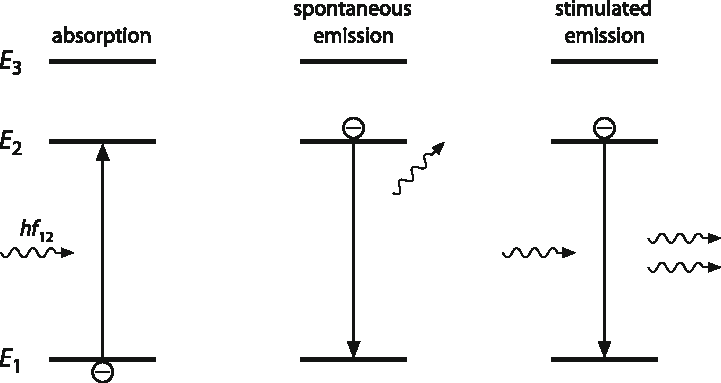
\includegraphics[width=0.65\textwidth]{content/graphics/processes.pdf}
	\caption{Schematic depiction of relevant processes inside the active medium. \cite{Eichler_2018}}
	\label{fig:processes}
\end{figure}

Raising the energy of an electron by $\Delta E = E_2 - E_1$ requires the annihilation of an incident photon that fulfills the condition
\begin{equation*}
	\Delta E = hf_{12} \: ,
\end{equation*}
where $h$ is the Planck constant. This process is referred to as absorption. The number of transitions per time and volume is proportional
to the density of ground state electrons $N_1$ as well as the photon flux or number per area and time $\varphi$ via
\begin{equation*}
	\left. \frac{dN_1}{dt} \right|_\text{ab} = -\sigma_{12} N_1 \varphi \: ,
\end{equation*}
with $\sigma_{12}$ denoting the effective cross section for absorbing a photon. From this also follows the typical exponential intensity
reduction
\begin{equation*}
	\left. \frac{dI}{dx} \right|_\text{ab} = -\sigma_{12} N_1 I \: ,
\end{equation*}
where $\alpha = -\sigma_{12} N_1$ gives the absorption coefficient.

When an atom is in an excited state, it returns to the ground state after a time interval, the duration of which follows some random
distribution with mean lifetime $\tau$. Due to its stochastic nature, this process is called spontaneous emission and has no predefined
direction or phase. The density in the higher level then follows
\begin{equation*}
	\left. \frac{dN_2}{dt} \right|_\text{sp} = - \tau^{-1} N_2 \: .
\end{equation*}

Besides this, emission can also be initiated by an incoming photon of appropriate frequency. This is called stimulated emission and results
in the production of radiation with the same energy, direction and phase as the inducing quantum. As the inverse process to absorption,
\begin{equation*}
	\left. \frac{dN_2}{dt} \right|_\text{st} = -\sigma_{21} N_2 \varphi \: ,
\end{equation*}
describes the time derivative and
\begin{equation*}
	\left. \frac{dI}{dx} \right|_\text{st} = \sigma_{21} N_2 I \: ,
\end{equation*}
the corresponding intensity relation. This means that stimulated emission leads to an increase in intensity, serving as a potential
mechanism for amplification when there are more electrons in the excited state than in the ground state and losses are compensated for.
This phenomenon in referred to as population inversion.

The cross sections can be identified with the Einstein coefficients $B_{ij}$ via
\begin{equation*}
	\sigma_{ij} = B_{ij} h f_{ij} / c \: ,
\end{equation*}
where $c$ is the speed of light in vacuo. Furthermore, for emission and absorption, the thermodynamic or quantum mechanical relation
\begin{equation*}
	\textsl{g}_1 \sigma_{12} = \textsl{g}_2 \sigma_{21}
\end{equation*}
holds, with $\textsl{g}_1$ and $\textsl{g}_2$ defining the degrees of degeneracy for the ground and excited states. Hereafter, it is
assumed that $E_1$ and $E_2$ have the same number of sublevels, so $\textsl{g}_1 = \textsl{g}_2$ for $\sigma_{12} = \sigma_{21}$ and
\begin{equation*}
	B \equiv B_{12} = B_{21} \: .
\end{equation*}
The reciprocal decay timescale defines another Einstein coefficient
\begin{equation*}
	A = \tau^{-1} \: ,
\end{equation*}
with which the stationary spectral radiance
\begin{equation*}
	\rho_s \equiv \pfrac{A}{B \,} = \frac{8\pi h f_{12}^3}{c^3}
\end{equation*}
can be written. Introducing the general spectral radiance
\begin{equation*}
	\rho = \varphi h f_{12} / c
\end{equation*}
and requiring $N = N_1 + N_2$ to be constant for a system of two energy levels, one finds
\begin{equation*}
	\frac{dN_1}{dt} = \left. \frac{dN_1}{dt} \right|_\text{ab} \!\! - \: \left. \frac{dN_2}{dt} \right|_\text{st} \!\! - \:
	\left. \frac{dN_2}{dt} \right|_\text{sp} \!\! = \: \rho B (N_2 - N_1) + AN_2 = - \frac{dN_2}{dt} \: .
\end{equation*}
For $\Delta N = N_2 - N_1$ then follows that
\begin{equation*}
	\pfrac{d\Delta N}{dt} = -2\frac{dN_1}{dt} = -2\rho B \Delta N - 2AN_2 + AN_1 - AN_1 = -2\rho B \Delta N - A\Delta N - AN \: .
\end{equation*}
After some time an equilibrium is reached inside the active medium, resulting in a vanishing time derivative. In this case, solving for the
stationary number difference
\begin{equation*}
	\Delta N_s = -\pfrac{AN}{A + 2\rho B} = -\pfrac{N}{1 + 2\rho / \kern-0.5pt \rho_s}
\end{equation*}
yields $\Delta N_s < 0$ for any system with only two energy levels.



\subsection{Necessity of multiple levels}

This result directly contradicts the requirement of population inversion $\Delta N_s > 0$ necessary for the amplification through stimulated
emission as discussed previously, preventing the usage of two level systems as the active medium. Adding more energy levels as depicted in
Figure \ref{fig:levels} solves this problem. Instead of immediately relaxing back to the ground state via spontaneous emission, excited
electrons now decay very quickly from $E_3$ to $E_2$ and $E_1$ to $E_0$ while the $E_2$ to $E_1$ transition takes longer. This means that
$A_{21} < A_{32}$ as well as $A_{21} < A_{10}$ and results in a distribution similar to what is shown below.

\begin{figure}[H]
	\centering
	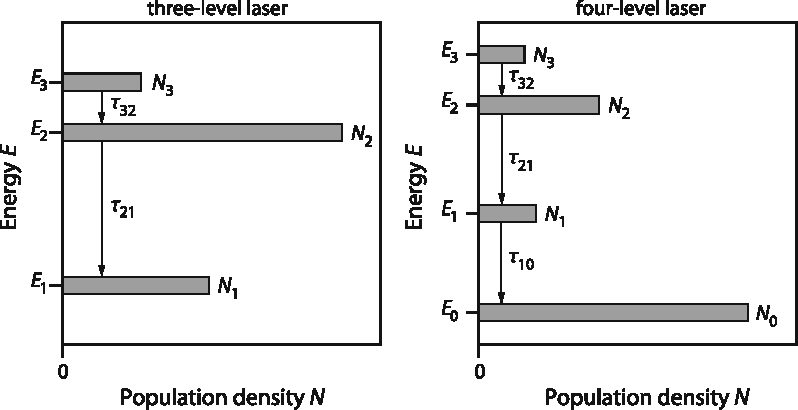
\includegraphics[width=0.70\textwidth]{content/graphics/levels.pdf}
	\caption{Exemplary energies and population densities for multiple levels. \cite{Eichler_2018}}
	\label{fig:levels}
\end{figure}

One then expects $N_0 \kern+0.5pt , N_2 \gg N_1 \kern+0.5pt , N_3$ for $N \approx N_0 + N_2$ and $\Delta N \approx N_2$ in the
stationary configuration. Accordingly, a population inversion $\Delta N_s > 0$ is trivial to achieve, making four level systems a suitable
choice for laser construction.

Such a system is realized by a \HeNe laser when the red mode at $\lambda = \qty{633}{\nano\meter}$ is used. Table \ref{tab:table} indicates
that this corresponds to a transition from the $3\symup{s}_2$ to the $2\symup{p}_4$ level, on which Figure \ref{fig:hene} provides more
detailed information.

\begin{table}[H]
	\centering
	\caption{Properties for different transitions of the \HeNe laser. \cite{Eichler_2018}}
	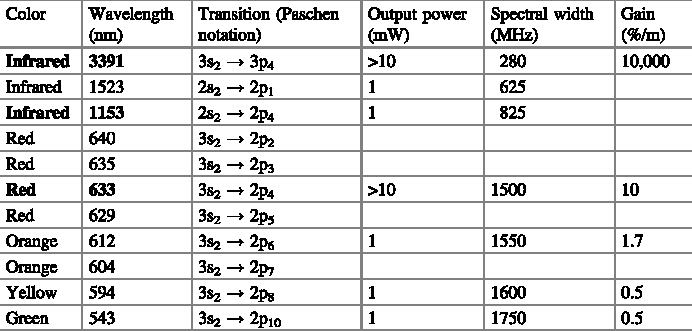
\includegraphics[width=0.85\textwidth]{content/graphics/table.pdf}
	\label{tab:table}
\end{table}

In this setup, the active medium is a mixture of helium and neon gases. Helium atoms are excited to metastable states via electric discharge
before colliding with neon atoms to provide excitation and transfer kinetic energy via 
\begin{equation*}
	\ce{He}^* + \ce{Ne} \longrightarrow \ce{He} + \ce{Ne}^* + E \: .
\end{equation*}
The excess energy $E \simeq \qty{100}{\milli\electronvolt}$ is dissipated as heat after the resonant transfer, as it measures about two times
the $\qty{300}{\kelvin}$ thermal energy. Due to the selection rules, the upper $2\symup{s}$ and $3\symup{s}$ levels have lifetimes of the order
$\qty{100}{\nano\second}$ because they can only decay to $\symup{p}$ levels, while lower states exhibit shorter $\qty{10}{\nano\second}$
timescales.

\begin{figure}[H]
	\centering
	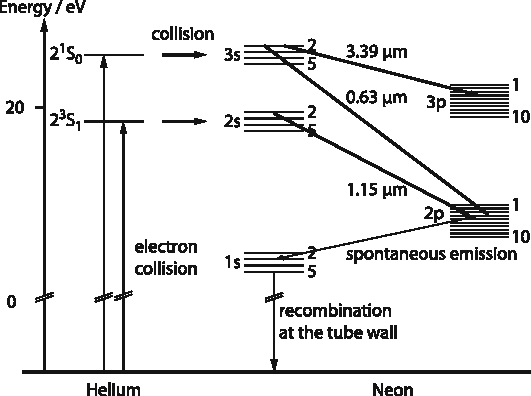
\includegraphics[width=0.60\textwidth]{content/graphics/hene.pdf}
	\caption{Energy level diagram of a \HeNe laser in Paschen notation. \cite{Eichler_2018}}
	\label{fig:hene}
\end{figure}



\subsection{Stability for different resonators}

To characterize spherical mirrors, the parameter
\begin{equation*}
	g_k = 1 - \pfrac{L}{R_k}
\end{equation*}
presents a convenient alternative to the curvature radii. With this, the radius $\textsl{w}_0$ at the waist of a Gaussian beam as depicted in
Figure \ref{fig:beam} can be calculated via
\begin{equation*}
	\textsl{w}_0^4 = \frac{\lambda^2 L^2 g_1 g_2 (1 - g_1 g_2)}{\pi^2 (g_1 + g_2 - 2 g_1 g_2)^2} \: .
\end{equation*}
It is immediately obvious that for $\textsl{w}_0$ to be a real solution,
\begin{equation*}
	0 \leq g_1 g_2 \leq 1
\end{equation*}
needs to hold, defining a stability condition for any mode to exist in a given resonator.

\begin{figure}[H]
	\centering
	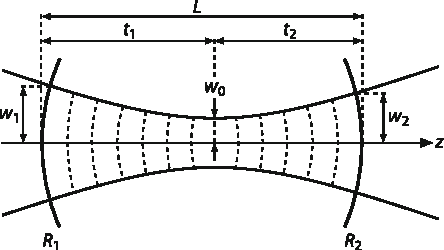
\includegraphics[width=0.47\textwidth]{content/graphics/beam.pdf}
	\caption{Adaptation of a Gaussian beam to a spherical mirror resonator. \cite{Eichler_2018}}
	\label{fig:beam}
\end{figure}

\begin{figure}[H]
	\centering
	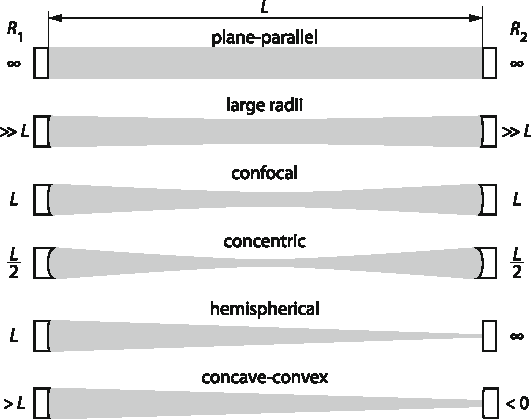
\includegraphics[width=0.56\textwidth]{content/graphics/resonators.pdf}
	\caption{Types of stable resonator configurations. \cite{Eichler_2018}}
	\label{fig:resonators}
\end{figure}

\begin{table}
	\centering
	\caption{Available mirrors for the construction of the cavity. \cite{hene}}
	\begin{tabular}{clrll}
		\toprule
		Mirror & \multicolumn{2}{c}{Design} & \multicolumn{2}{c}{Surface} \\
		\midrule
		planar  & $R_1 = \infty$ & flat $\mathbin{/}$ flat & HR (high reflectivity) & $R \geq \qty{99}{\percent}$ \\
		concave & $R_1 = \qty{1000}{\milli\meter}$ & spherical $\mathbin{/}$ flat & HR (high reflectivity) & $R \geq \qty{99}{\percent}$ \\
		concave & $R_1 = \qty{1400}{\milli\meter}$ & spherical $\mathbin{/}$ flat & HR (high reflectivity) & $R \geq \qty{99}{\percent}$ \\
		concave & $R_2 = \qty{1400}{\milli\meter}$ & spherical $\mathbin{/}$ flat & OC (out coupling) & $T \simeq \qty{2}{\percent}$ \\
		\bottomrule
	\end{tabular}
	\label{tab:config}
\end{table}

Figure \ref{fig:resonators} displays some realizable mirror configurations, while Table \ref{tab:config} lists available parts for the
setup at hand. Their stability factors are evaluated graphically in Figure \ref{fig:stability} to determine the maximum possible resonator
length.

\begin{figure}[H]
	\centering
	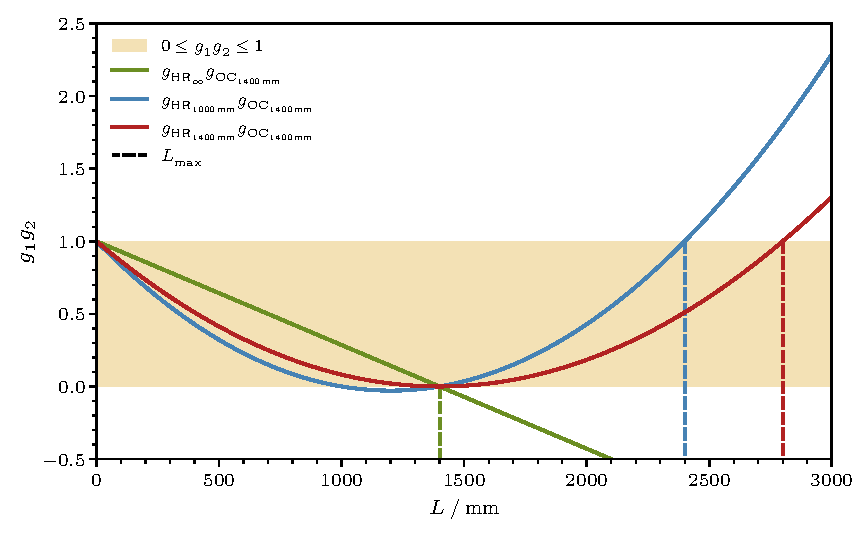
\includegraphics{build/stability.pdf}
	\caption{Stability diagram as functions of the resonator length.}
	\label{fig:stability}
\end{figure}

It should be noted that an unstable resonator with $g_1 g_2 < 0$ or $g_1 g_2 > 1$ does not necessarily preclude laser operation. Unstable
lasing implies large diffraction losses, as significant parts of laser power leak around the mirror edges, in turn requiring high optical
gain in the active medium to compensate. The resulting configuration can however be less sensitive to disturbances such as thermal lensing
or misalignment than a stable resonator, providing desirable properties depending on the application.



\subsection{Transverse and longitudinal modes}

During normal operation, different transverse electromagnetic modes $(\text{TEM})$ interfere in the plane perpendicular to the beam axis.
Their orders are denoted using indices like $\text{TEM}_{r\vartheta}$ and $\text{TEM}_{xy}$ to give the integer number of nodes in direction
of the respective coordinate. Assuming a Gaussian beam profile, circular symmetry can be parametrized by multiplication with Laguerre
polynomials. If modes are selected using a thin wire as is the case here, a rectangular symmetry is required. A cut of the electric field
strength in $x$ direction then follows
\begin{equation*}
	E_n (\xi) = H_m (\xi) e^{-\xi^2 / 2} \: ,
\end{equation*}
where $H_m (\xi)$ is the appropriate Hermite polynomial and $\xi = \sqrt{2} \, x / \textsl{w}_0$ connects the parameter to the spacial
coordinate. The first three solutions
\begin{align*}
	H_0 = 1 \: , && H_1 (\xi) = 2 \xi \: , && H_2 (\xi) = 4 \xi^2 - 2
\end{align*}
lead to the patterns shown in Figure \ref{fig:modes} below.

\begin{figure}[H]
	\centering
	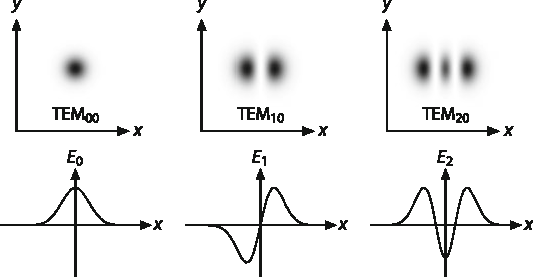
\includegraphics[width=0.55\textwidth]{content/graphics/modes.pdf}
	\caption{Observable $\text{TEM}_{xy}$ modes for rectangular geometry. \cite{Eichler_2018}}
	\label{fig:modes}
\end{figure}

% \begin{figure}[H]
% 	\centering
% 	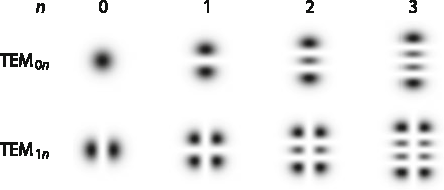
\includegraphics[width=0.50\textwidth]{content/graphics/rect.pdf}
% 	\caption{Select $\text{TEM}_{xy}$ modes for rectangular geometry. \cite{Eichler_2018}}
% 	\label{fig:rect}
% \end{figure}

% \begin{figure}[H]
% 	\centering
% 	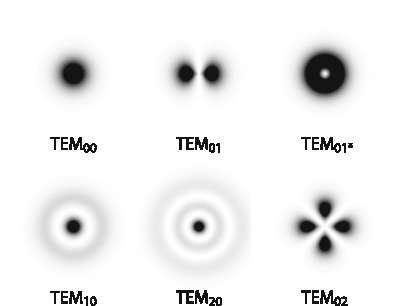
\includegraphics[width=0.45\textwidth]{content/graphics/circ.pdf}
% 	\caption{Select $\text{TEM}_{r\vartheta}$ modes for circular geometry. \cite{Eichler_2018}}
% 	\label{fig:circ}
% \end{figure}

Obtaining the intensity, which is the quanitity that is actually measured, requires squaring the absolute value of the electric field
amplitude. From $I \propto |E|^2$ follows
\begin{align}
	I_{\text{TEM}_{00}} (x) &= I_{00} e^{-2 x^2 / \textsl{w}_0^{\, 2}} \: , \\
	I_{\text{TEM}_{10}} (x) &= I_{10} x^2 e^{-2 x^2 / \textsl{w}_0^{\, 2}} / \textsl{w}_0^{\, 2} \: , \\
	I_{\text{TEM}_{20}} (x) &= I_{20} (4 x^2 / \textsl{w}_0^{\, 2} - 1)^2 e^{-2 x^2 / \textsl{w}_0^{\, 2}}
	\label{eqn:TEMEQN}
\end{align}
as the theoretically expected distributions with arbitrary normalization factors. Additional degrees of freedom may be introduced to
account for distortive effects such as a finite background or an asymmetric shape due to inaccurate centering of the probe.

In multimode operation, longitudinal modes in direction of beam expansion instead interfere to produce beating patterns in the signal.
This is due to slight frequency variations that result from the multiple allowed standing wave solutions inside the resonator.



\subsection{Doppler broadening of the transition}
\label{sec:doppler}

This beating pattern is quite complicated, but can be analyzed by decomposing it to its Fourier coefficients. From $L = m\lambda / 2$
for standing waves follows $f = mc / 2L$ or
\begin{equation}
	\Delta f_\text{PP} = \pfrac{c}{2L}
	\label{eqn:bla}
\end{equation}
as the distance between spectral peaks, which is proportional to the reciprocal resonator length with
$\Delta f_\text{PP} \simeq \qty{100}{\mega\hertz}$ as a typical value. Additionally, the uncertainty principle requires energy levels
to have $\Delta E = h / 2\pi \tau$ as a finite width. A natural linewidth
\begin{equation*}
	\Delta f_\text{N} = \pfrac{1}{2\pi}
	\left( \pfrac{1}{\raisebox{0.55ex}{$\tau_1$}} + \pfrac{1}{\raisebox{0.55ex}{$\tau_2$}} \right)
\end{equation*}
is the result, which describes a Lorentzian profile
\begin{equation*}
	F_\text{N} (f) = \frac{(\Delta f_\text{N} / 2)^2}{(f - f_{12})^2 + (\Delta f_\text{N} / 2)^2} \: .
\end{equation*}
Values are of the order $\Delta f_\text{N} \simeq \qty{10}{\mega\hertz}$ for a \HeNe laser. A homogenous broadening is introduced from
elastic collisions, which cause phase shifts during emission. The width
\begin{equation*}
	\Delta f_\text{C} = \sqrt{\pfrac{3}{4mkT \,}} \, d^2 p
\end{equation*}
follows from thermodynamics and has values around $\Delta f_\text{C} \simeq \qty{100}{\mega\hertz}$ at temperatures of
$T = \qty{300}{\kelvin}$ with the Boltzmann constant $k$ as well as $m$ and $d$ as the mass and diameter of the atoms.

\begin{figure}[H]
	\centering
	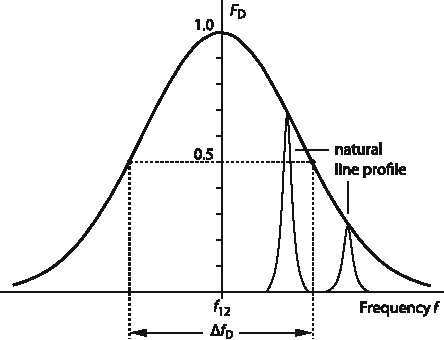
\includegraphics[width=0.60\textwidth]{content/graphics/broadening.pdf}
	\caption{Typical Doppler broadening compared to natural line width. \cite{Eichler_2018}}
	\label{fig:broadening}
\end{figure}

Lastly, the motion of emitting particles inhomogenously shortens or lengthens the emitted wavelength according to the Doppler effect.
This can be written for $v \ll c$ as
\begin{equation*}
	f_{12}' = f_{12} (1 \pm v / c) \: ,
\end{equation*}
with the sign indicating movement towards or away from the detector. In case of thermal equilibrium, this obeys Maxwell statistics with
a Gaussian line shape function
\begin{equation*}
	F_\text{D} (f) = 2^{- 4 (f - f_{12})^2 / \Delta f_\text{D}^2}
\end{equation*}
and a full width half maximum
\begin{equation}
	\Delta f_\text{D} = 2 f_{12} \sqrt{2kT \ln 2 / m} / c \: .
	\label{eqn:fwhm}
\end{equation}
Due to values around $\Delta f_\text{D} \simeq \qty{1.5}{\giga\hertz}$ for a \HeNe laser, the Gaussian represents an enveloping function
with much larger spread than other contributions as can be seen in Figure \ref{fig:broadening}.



\subsection{Brewster window and polarization}

Inserting a Brewster plate at the Brewster angle inside the cavity before the mirror as shown in Figure \ref{fig:setup} allows the light
component with polarization parallel to the plane of incidence to be transmitted with zero losses due to vanishing reflectivity, while
about $\qty{20}{\percent}$ of the orthogonally polarized intensity are reflected and therefore lost. Due to the nonlinear operation of
a laser and by assuming losses per cycle of $\qty{2}{\percent}$ at the out coupler as well as a gain around $\qty{10}{\percent}$ inside
the active medium, one finds that only the parallel part is capable of lasing, making the output fully linearly polarized.

\begin{figure}[H]
	\centering
	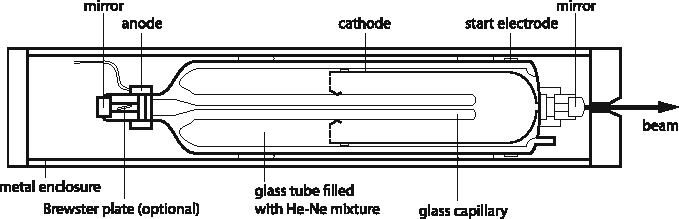
\includegraphics[width=0.90\textwidth]{content/graphics/setup.pdf}
	\caption{Schematic setup of a \HeNe laser generating polarized output. \cite{Eichler_2018}}
	\label{fig:setup}
\end{figure}

The intensity of a polarized beam decreases on a perfect polarizer according to Malus
\begin{equation}
	I(\theta) = I_0 \cos^2\theta \: ,
	\label{eqn:pol}
\end{equation}
with $\theta$ giving the angle between the initial polarization and the polarizer axis.



% \subsection{Wavelength from the diffraction pattern}
